\documentclass{article}
\documentclass[AER, draftmode]{AEA}
\usepackage{graphicx} %package to manage images
\graphicspath{ {./figures/} }
\usepackage{hyperref}
\usepackage{caption}
\usepackage[font=scriptsize]{subcaption}
\captionsetup[figure]{labelsep=none}
\captionsetup[table]{labelsep=none}
\usepackage{bbm}
\usepackage{amsmath}
\usepackage{import}
\usepackage{array}
\usepackage{booktabs}
\usepackage{afterpage}
\usepackage{floatrow}
\usepackage{pdflscape}
\usepackage{soul}
\usepackage{float}
\usepackage{adjustbox}
\usepackage{longtable}


\title{trends in health in pregnancy (overleaf)}
\author{Sidh Pandit}
\date{April 2025}

\begin{document}

\maketitle

\section{Introduction}


\begin{figure}[H]
    \centering
    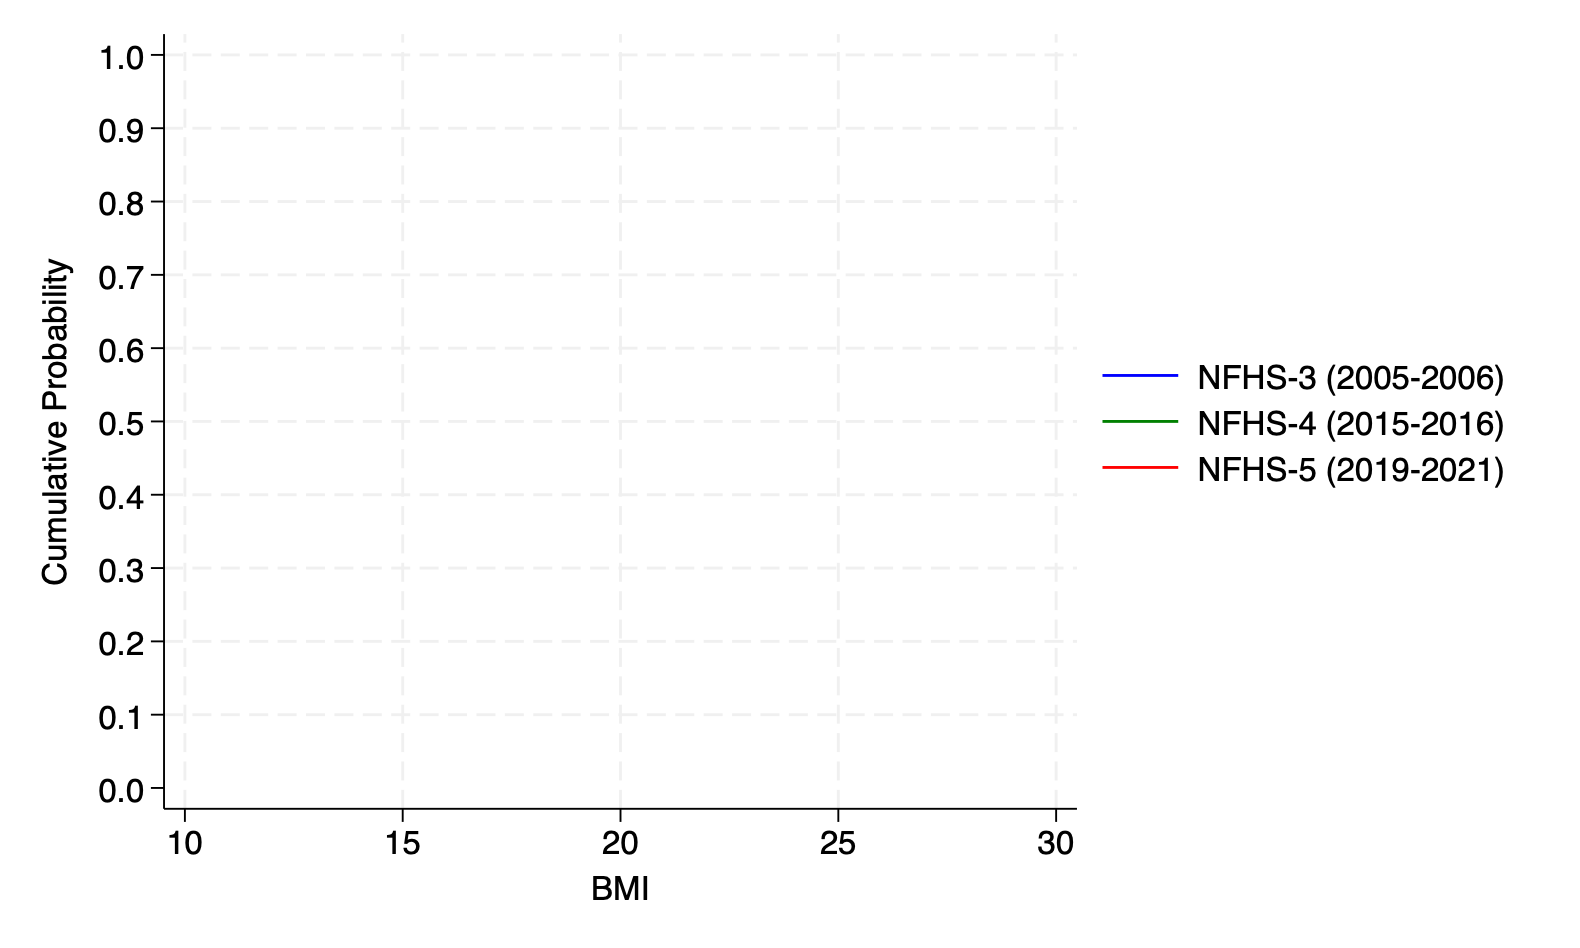
\includegraphics[width=\textwidth]{figures/cdf prepregnancy bmi.png}
    \caption{: testing the caption feature}
    
\end{figure}



\begin{figure}[H]
    \centering
    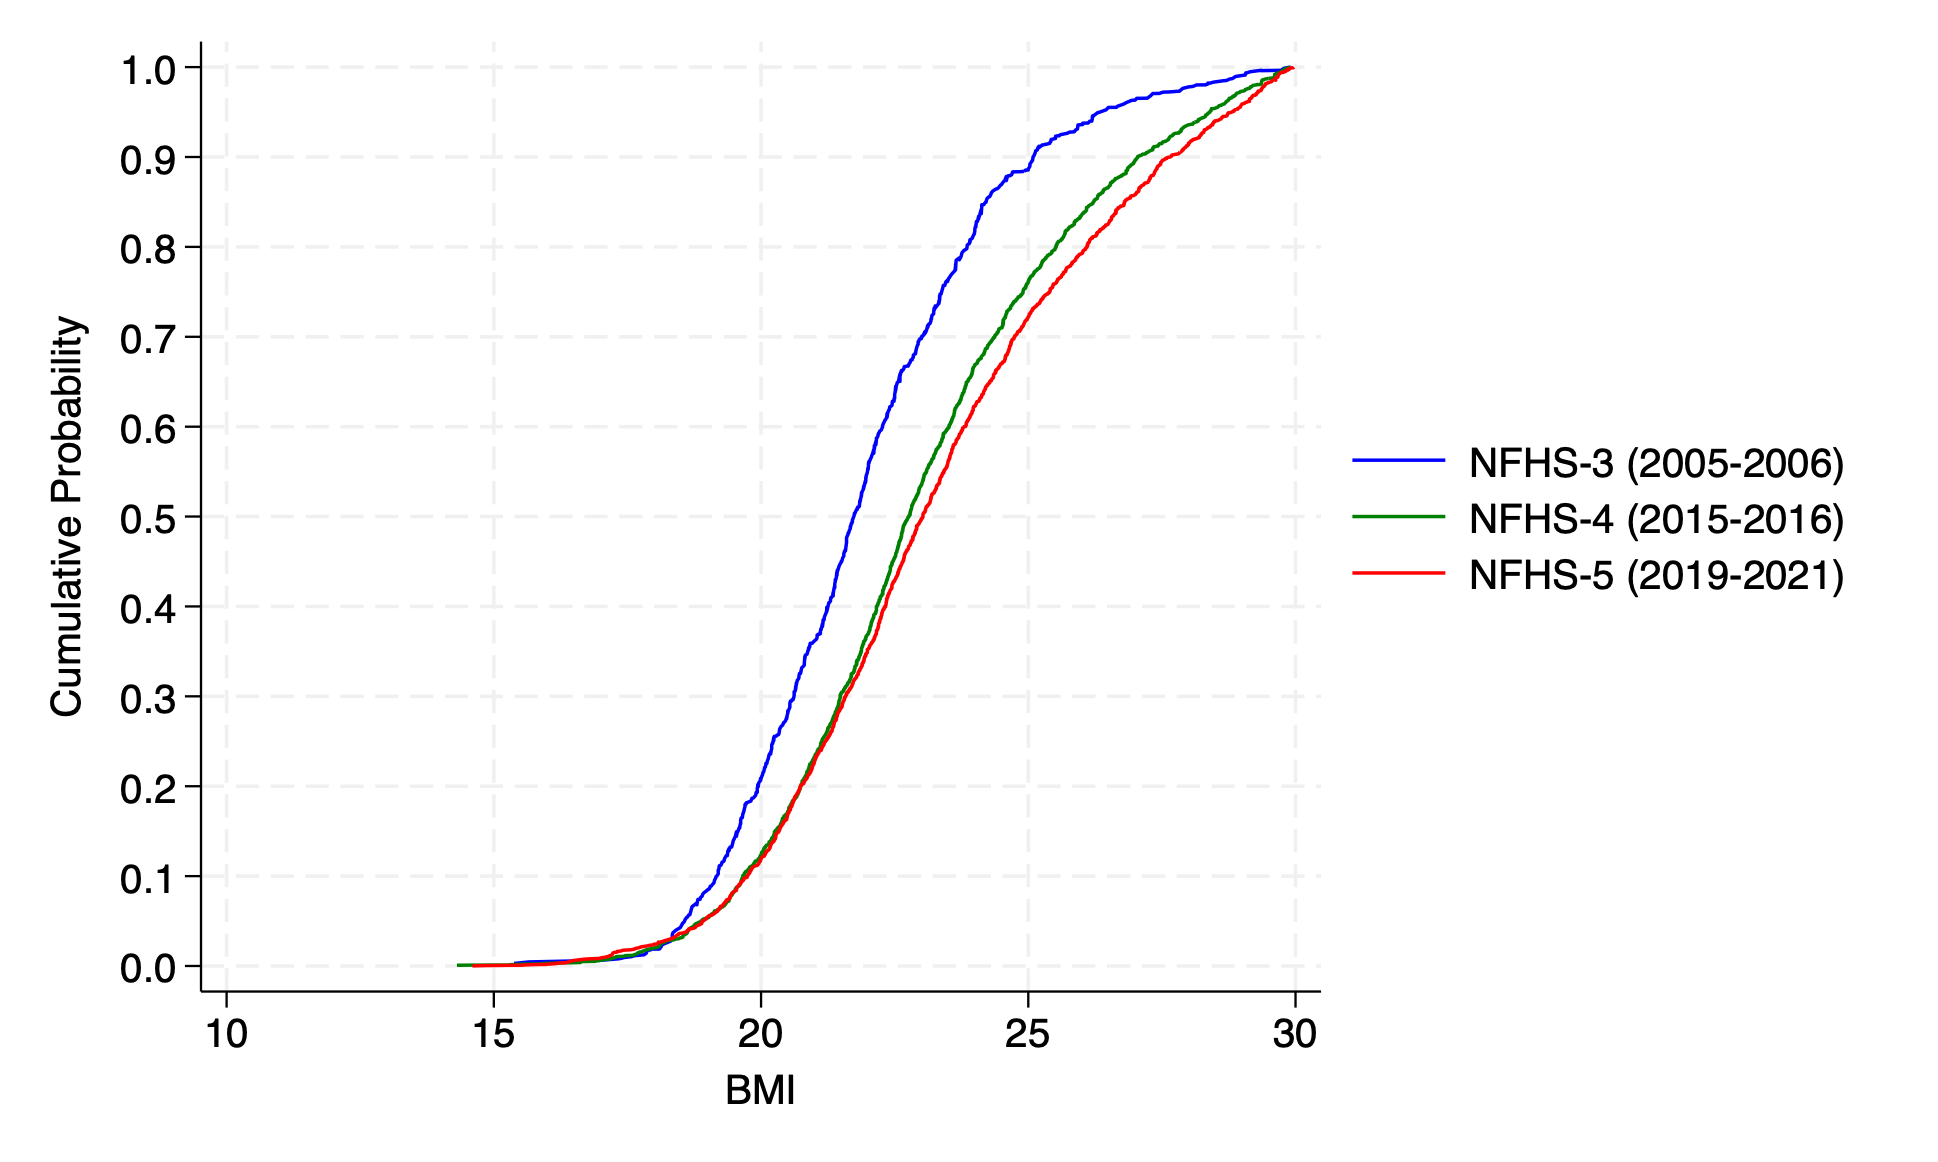
\includegraphics[width=\textwidth]{figures/cdf nine months bmi.png}
    \caption{: testing the caption feature}
    
\end{figure}


\begin{figure}[H]
    \centering
    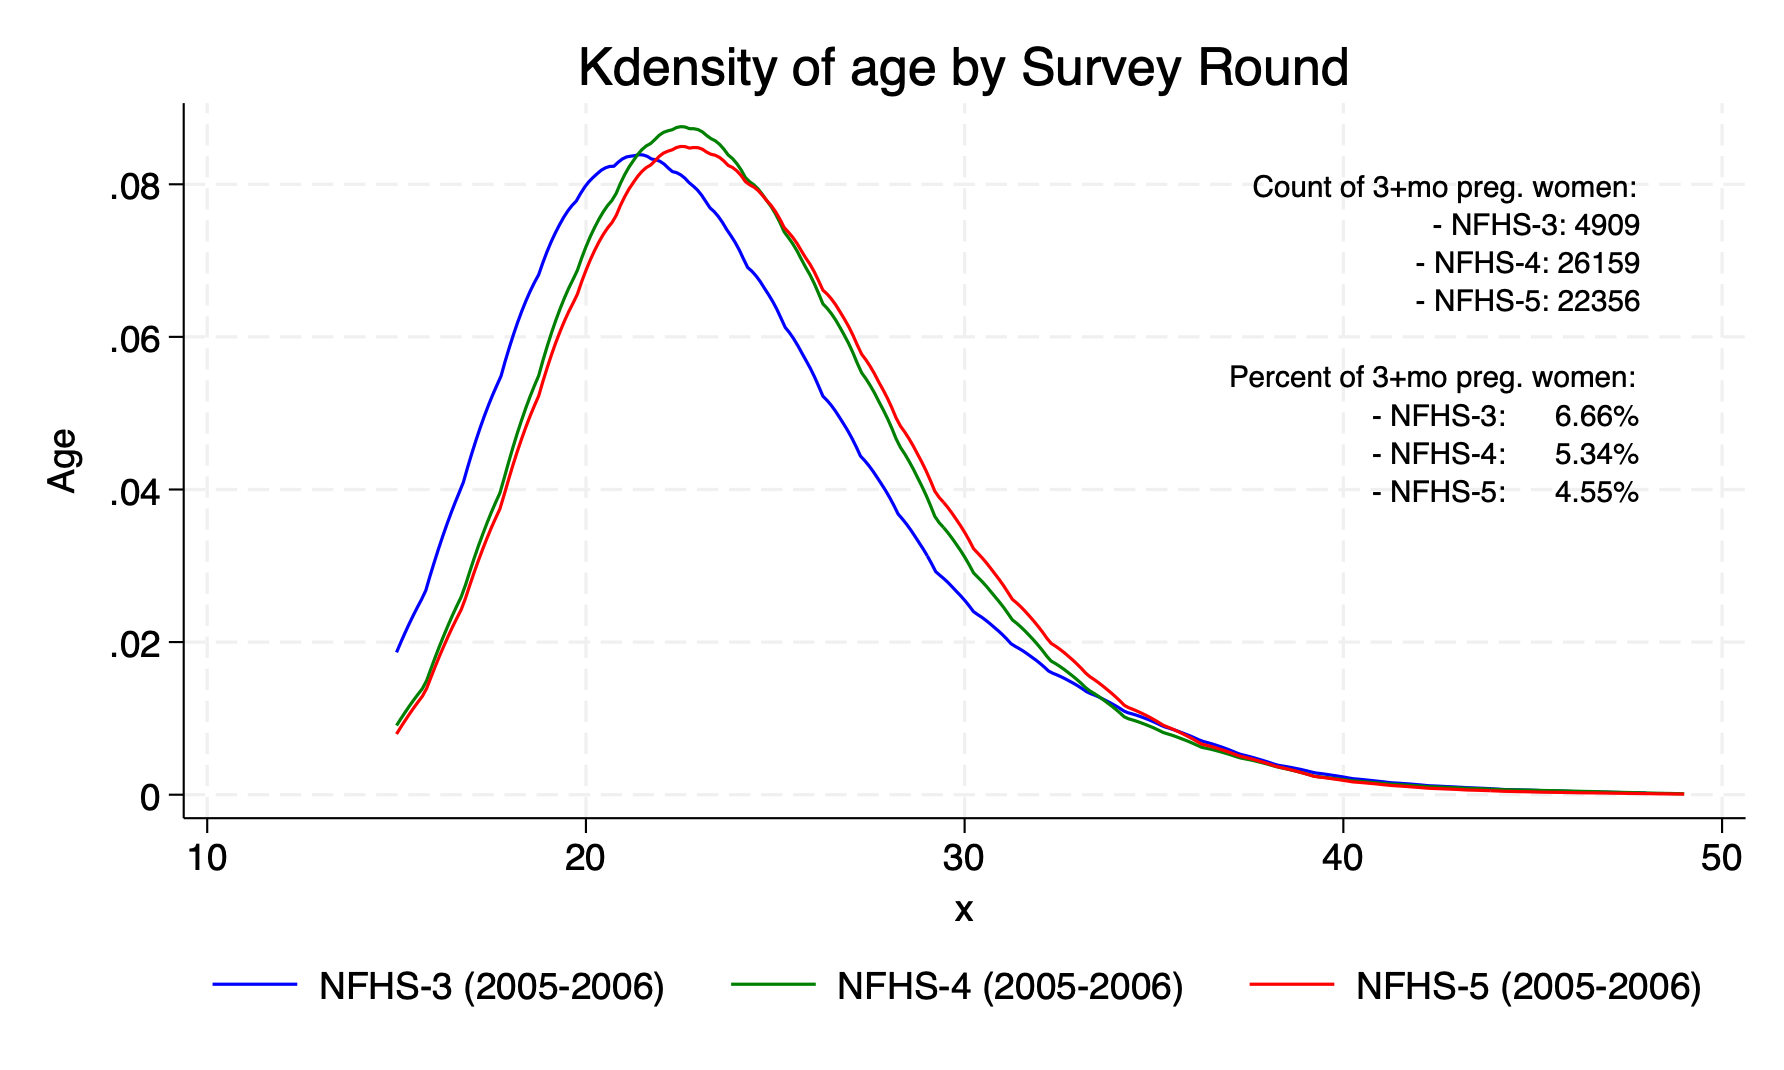
\includegraphics[width=\textwidth]{figures/kdensities ages.png}
    \caption{: testing the caption feature}
\end{figure}


\begin{figure}[H]
    \centering
    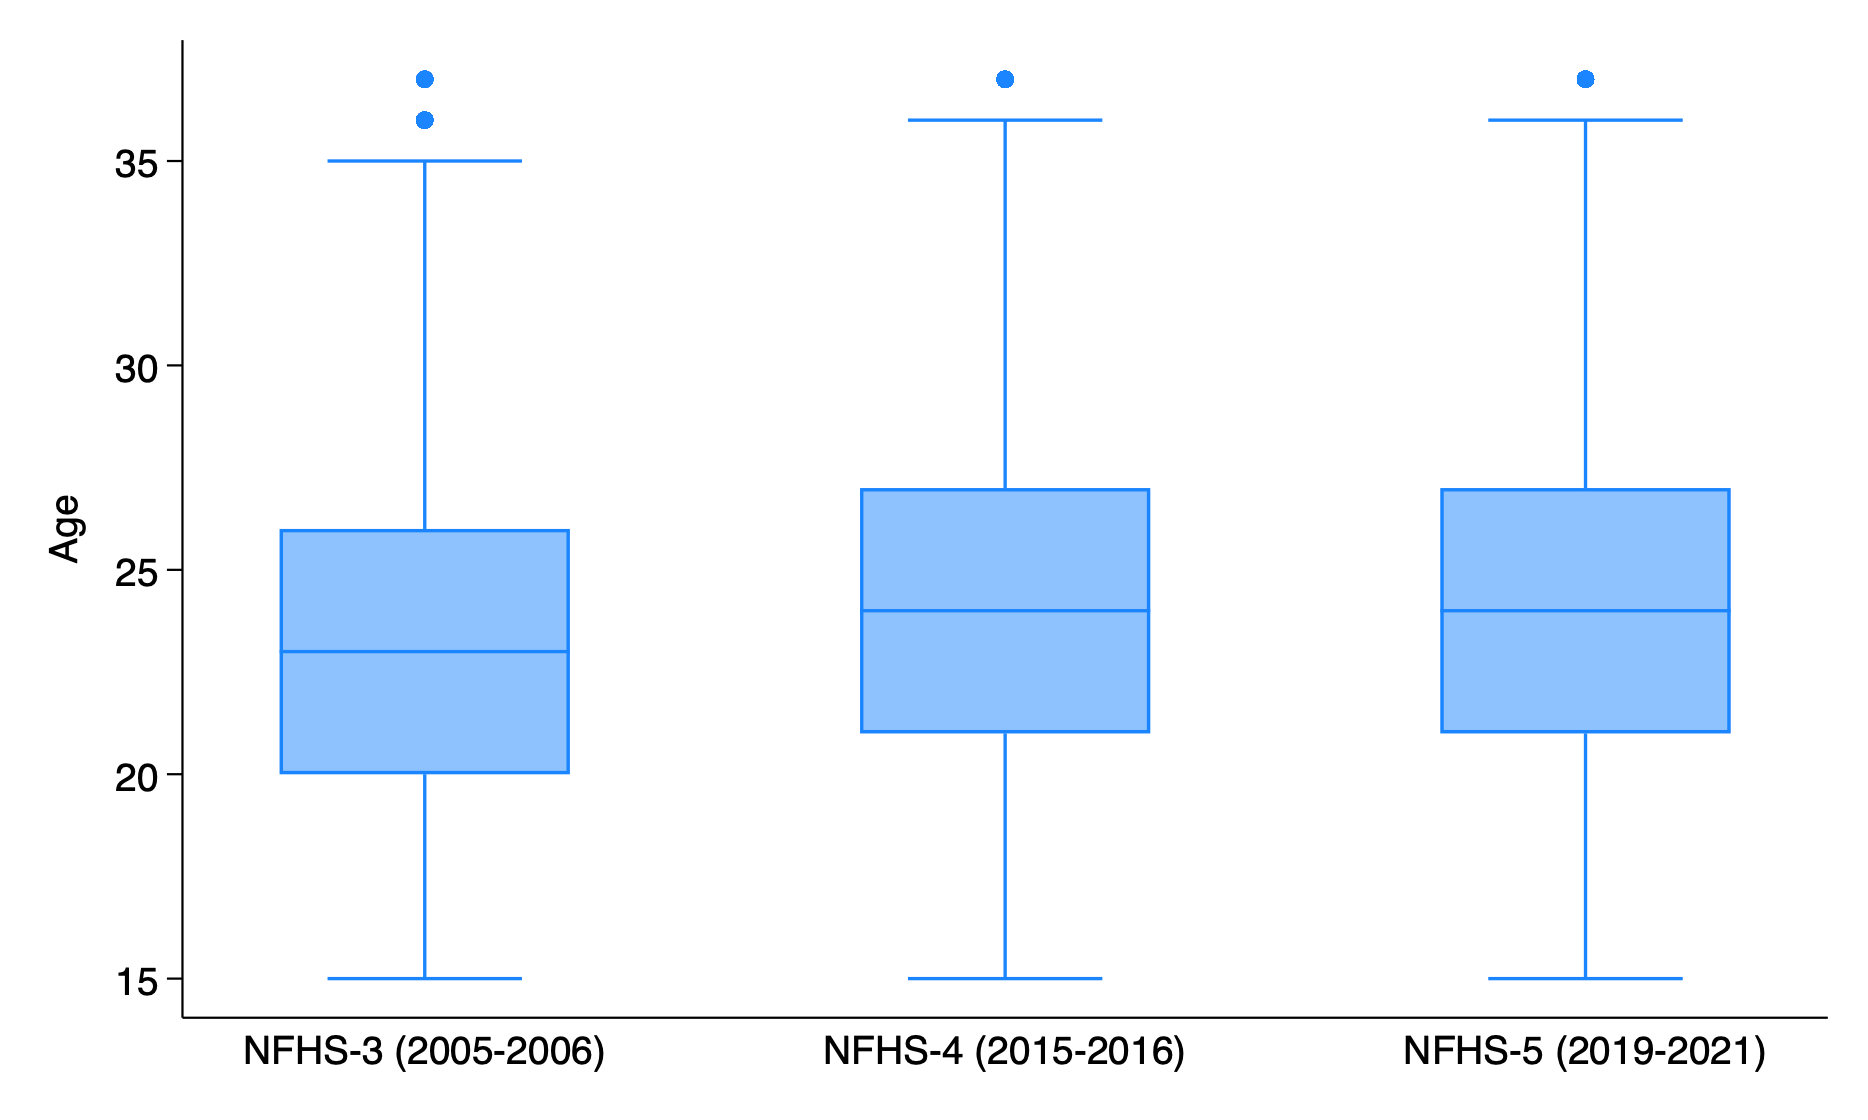
\includegraphics[width=\textwidth]{figures/boxplots ages.png}
    \caption{: testing the caption feature}
\end{figure}

\begin{figure}[H]
    \centering
    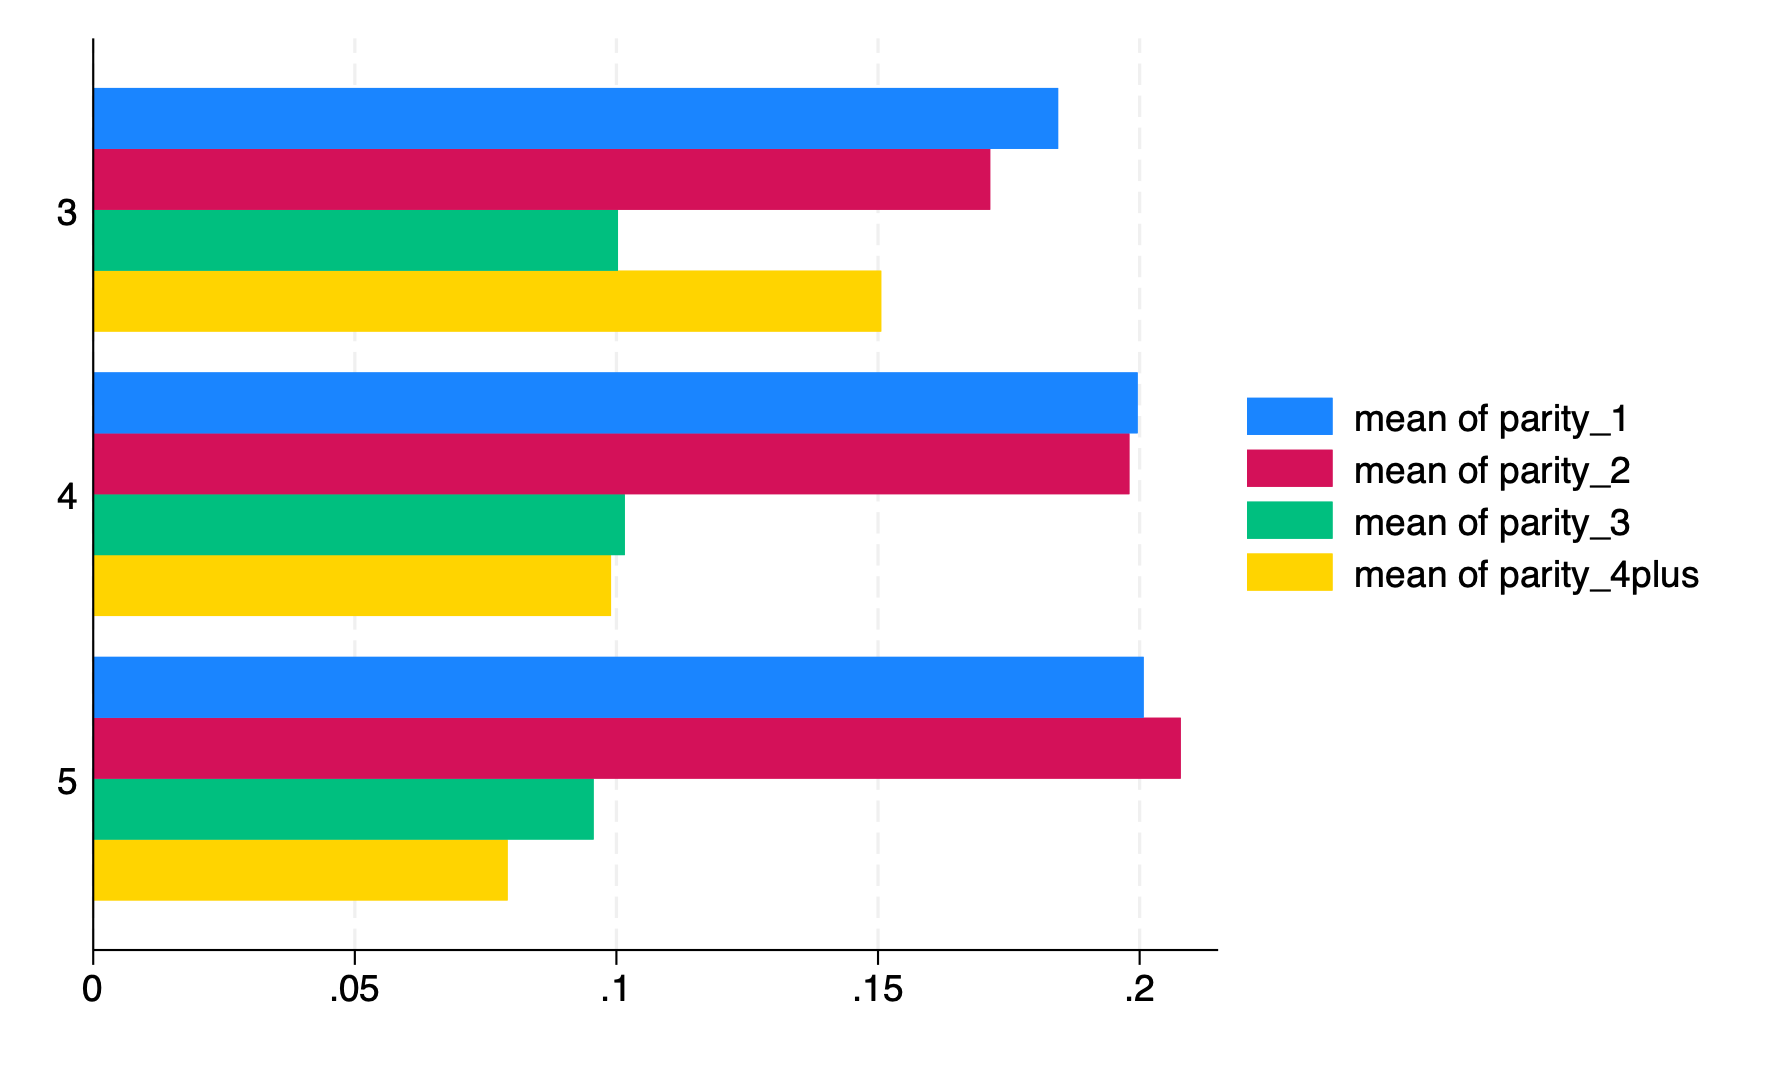
\includegraphics[width=\textwidth]{figures/bar graph number of children.png}
    \caption{: testing the caption feature}
\end{figure}

\end{document}



fix lines on end-pregnancy BMI
remove titles on graphs from stata
label xaxis on kdensity age
maybe make stats on kdensity age separate table


